% Observed retrospective fits; prospective GPU/accuracy cells remain unmeasured.
\subsection{Prospective comparison of accuracy and memory}
\label{sec:expert-memory-study}

We specify a static comparison at one expert-memory point: native execution,
state-balanced retention, pooled labelled-token frequency retention and one
matched random keep-set. The planning target removes 25\% of routed-expert
bytes. Each routed layer retains respectively 24, 96, 192, 192, 96, 48 and 96 experts
for GPT-OSS, Nemotron, Qwen3.5, Qwen3.6, Gemma, GLM and Qwen3-30B. The inspected
checkpoint headers give equal serialized bytes per expert within each model,
so these quotas retain 75\% of its serialized routed-expert bytes. This is a
projection, not a GPU-residence measurement; dense and shared paths remain.

Five common retrospective folds group the 1,547 historical questions into
1,486 duplicate families. A family has total weight one, shared equally among
its member questions. For class $c$, layer $\ell$ and expert $e$, first average
selected-slot counts over questions within family $f$, giving $C_{fc\ell e}$.
The state-balanced score is
\begin{equation}
 s^{\mathrm{bal}}_{\ell e}
 =\frac{1}{|\mathcal C|}\sum_{c\in\mathcal C}
   \frac{1}{|\mathcal F_c|}\sum_{f\in\mathcal F_c}
   \frac{C_{fc\ell e}}{\sum_j C_{fc\ell j}},
\end{equation}
where $\mathcal F_c$ contains training families with observed class $c$.
Every class requires training support. The frequency control pools the same
family-weighted labelled counts, proportional to their observed token mass:
\begin{equation}
 s^{\mathrm{freq}}_{\ell e}
 =\frac{\sum_{f,c}C_{fc\ell e}}{\sum_{f,c,j}C_{fc\ell j}}.
\end{equation}
Both methods use identical layer/group quotas and break ties by original
expert ID. Random priorities use seed 20261008 and fix one set per model;
comparisons are conditional on those sets. Fold-held-out class/layer coverage,
minimum coverage, mask overlap and fold stability are retrospective analysis
endpoints. All-reasoning frequency is only an offline sensitivity. We make no
quality claim against conventional all-token or output-aware pruning.
Final masks use the complete historical corpus before pilot outcomes are
available, without correctness ranking or a mask sweep.

The complete five-fold analysis is now observed for all seven models
(Figure~\ref{fig:expert-memory-heldout}). State balancing has higher minimum
class coverage than pooled labelled frequency in every fold for GPT-OSS,
Nemotron, Gemma, GLM and Qwen3-30B. Pooled labelled frequency is higher in every
fold for Qwen3.5 and Qwen3.6. These are held-out routing-slot coverage
observations; they establish neither benchmark accuracy nor accuracy retention
after physical removal. The fixed random masks have minimum class coverage
between 73.4\% and 77.2\% across the model/fold cells. The displayed fold spread
describes partition stability and is not a confidence interval.

\begin{figure}[t]
\centering
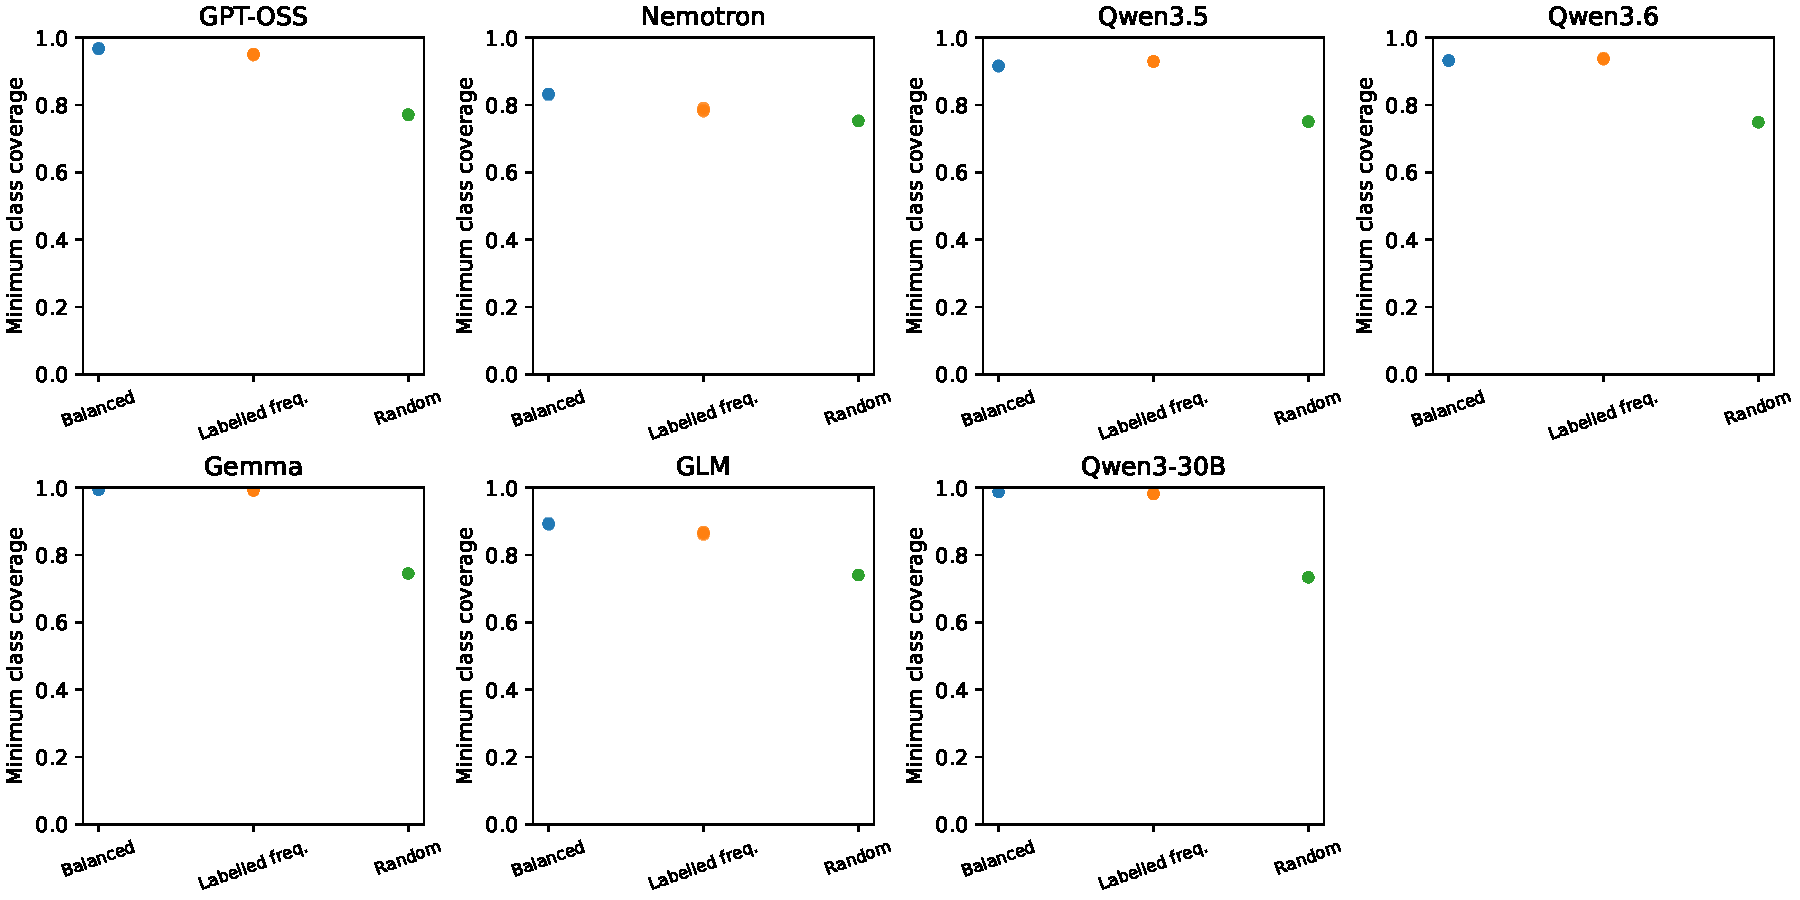
\includegraphics[width=\linewidth]{figures/expert_memory_heldout_r2.pdf}
\caption{Minimum held-out reasoning-class coverage at 75\% expert retention.
Each point is one common duplicate-family fold; coverage averages routed layers
within class before taking the minimum over classes. Selection uses training
folds only and identical quotas for state balancing, pooled labelled frequency
and fixed random controls.}
\label{fig:expert-memory-heldout}
\end{figure}

The consecutive-sentence analysis also now covers all seven models on the
common 522-question/509-family population
(Figure~\ref{fig:expert-memory-transitions}). An edge requires consecutive
original sentence indices in the same reasoning segment; gaps and missing
labels break adjacency. Labelled-sentence coverage ranges from 7.0\% for
Qwen3.6 to 28.1\% for GPT-OSS. The matrices therefore describe observed labelled
adjacencies rather than complete reasoning trajectories. Cell/source family
support, coverage denominators and endpoint-censored dwell durations accompany
the saved transition receipt.

\begin{figure}[t]
\centering
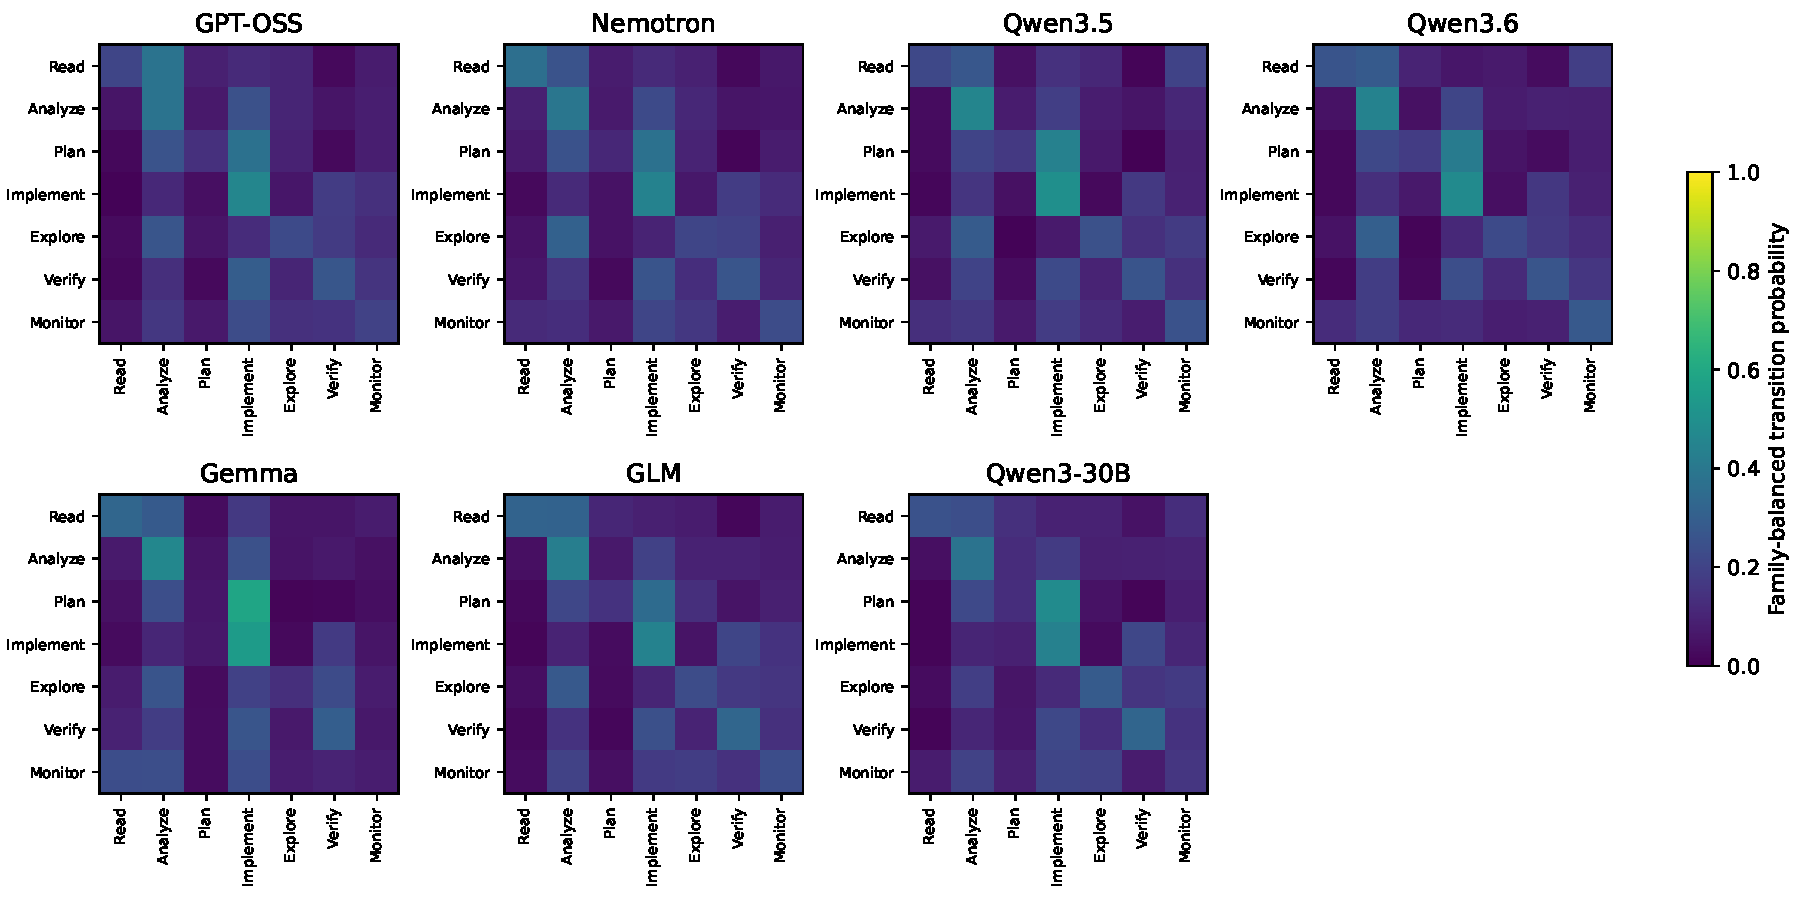
\includegraphics[width=\linewidth]{figures/expert_memory_transitions_r2.pdf}
\caption{Family-balanced next-class probabilities for consecutive observed
sentences, using the common 509-family population. Rows are current classes
and columns are next classes. Missing labels and sentence gaps break adjacency;
unsupported rows are missing.}
\label{fig:expert-memory-transitions}
\end{figure}

The separate private loader preserves original router dimensions and native
selection, masks unavailable logits and selection correction biases, and
maps original selected IDs to compact expert allocations. It streams retained
weights and packed quantization metadata from the original checkpoints.
Qualification compares full-resident masked and compact execution at identical
hidden states for prefill/decode in every routed layer. Routing-weight
tolerances are absolute $10^{-6}$ and relative $10^{-5}$; BF16 output tolerances
are absolute and relative $10^{-2}$. Unique expert storage must fall, with zero
removed-expert dispatch, unchanged native backend/precision, valid cleanup
and equal resolved KV/hybrid-state cache specifications across arms. Allocator
allocation/reservation, process GPU residence and load/decode peaks are
distinct reported quantities. No cross-run sampled-token replay is required.

Prospective generation uses native model sampling, one seed per test family,
output cap 32,768 and context 40,960. Inputs may not silently reduce this cap.
The frozen full-MATH duplicate graph excludes historical families and the
128-family verification reservation, leaving 4,351 families before later-exposure
reconciliation. The completed roster reconciliation excludes no additional
eligible family. A proportional subject/level order selects one representative
per family. Thirty-two fresh pilot families are excluded from the final test.
Pricing assignments remain in that pilot, and identical frozen policies alias
receipts rather than duplicate generation. Fresh native controls are required
because the new runtime/cap differs from the historical benchmarks.

Let $q_U$ be the maximum simultaneous one-sided exact binomial upper bound for
paired score discordance over the 21 state-balanced-versus-control contrasts.
The blinded sizing rule fixes
\begin{equation}
 N=32\left\lceil\frac{3.038^2q_U}{0.05^2\times32}\right\rceil,
\end{equation}
giving 640--3,712 final independent families at a five-percentage-point planning
half-width. Unknown pilot semantic pairs count conservatively as discordant.
There is no accuracy-retention margin. All-assignment strict benchmark scores
and semantic-correctness bounds retain caps, absent final answers, execution
failures and uncapped unresolved grades. Final inference resamples the same
families across models for 21 simultaneous paired contrasts; degenerate
resampling cannot produce a zero-width confidence interval. The reported
point must measure realized expert/total memory jointly with accuracy.

The harness and synthetic contracts are implemented; all-seven retrospective
fits and transitions are observed and final masks are frozen. GPU qualification,
realized-memory measurements and pilot/final accuracy remain unmeasured.
The all-seven qualification allocations are authorized and accepted with a
224 billing core-hour/28 GPU-hour ceiling; this is an engineering reservation,
not a measured production price. Final computation requires measured prices and
complete entitlement, storage and deadline feasibility; infeasible precision
is reported without silently reducing $N$.
